\documentclass[12pt]{article}



\usepackage{fullpage}
\usepackage[spanish]{babel}
\usepackage{amsfonts} %for double trace letters
\usepackage{amssymb}
\usepackage{amsmath} %for special/unusual mathematical characters
\usepackage{eufrak} %for gothic letters
\usepackage{graphicx} %Image includer package
\graphicspath{{Images/}} %Image directory
\usepackage{xcolor}

\usepackage{multicol} %For writing text in columns
\setlength{\columnsep}{1cm} %Defines separation of columns

\usepackage{tcolorbox} %for boxes that enclose text
\usepackage{color}
\definecolor{myblue}{rgb}{.8, .8, 1}

\usepackage{empheq}

\newlength\mytemplen
\newsavebox\mytempbox

\makeatletter
\newcommand\mybluebox{%
    \@ifnextchar[%]
       {\@mybluebox}%
       {\@mybluebox[0pt]}}

\def\@mybluebox[#1]{%
    \@ifnextchar[%]
       {\@@mybluebox[#1]}%
       {\@@mybluebox[#1][0pt]}}

\def\@@mybluebox[#1][#2]#3{
    \sbox\mytempbox{#3}%
    \mytemplen\ht\mytempbox
    \advance\mytemplen #1\relax
    \ht\mytempbox\mytemplen
    \mytemplen\dp\mytempbox
    \advance\mytemplen #2\relax
    \dp\mytempbox\mytemplen
    \colorbox{myblue}{\hspace{1em}\usebox{\mytempbox}\hspace{1em}}}

% for theorems
\usepackage{amsthm}
 
\theoremstyle{definition}
\newtheorem{definition}{Definici\'on}[section]

\theoremstyle{theorem}
\newtheorem{theorem}{Teorema}[section]

\theoremstyle{corolary}
\newtheorem{corolary}{Corolario}[section]

\DeclareMathOperator{\Arg}{Arg}
\DeclareMathOperator{\Log}{Log}
\DeclareMathOperator{\sen}{sen}
\DeclareMathOperator{\senh}{senh}
\DeclareMathOperator{\tg}{tg}
\DeclareMathOperator{\ctg}{ctg}
\DeclareMathOperator{\tgh}{tgh}
\DeclareMathOperator{\ctgh}{ctgh}
\DeclareMathOperator{\sech}{sech}
\DeclareMathOperator{\csch}{csch}


\begin{document}

	\title{Transformaciones}
	\author{Breggia, Bruno M.}
	\date{}
	\maketitle

\begin{center}
	
\includegraphics[scale=0.4]{vajilla2.jpg}
	
	\textit{``Porque del polvo eres, y al polvo volver\'as"}\\
	\textbf{G\'enesis} 3:19
\end{center}

%No seremos magos ni hechiceros, pero 
Con las herramientas del c\'alculo complejo contamos con la capacidad de, mediante una funci\'on cualquiera, transformar un punto en el plano complejo a otro. Esto es, si vemos a las funciones como teletransportadores que desplazan instant\'aneamente puntos de un lugar en el plano a otro, somos capaces de revolver el plano complejo a gusto. Gran cosa... dir\'an sarc\'asticamente. Pero punto por punto, curva por curva, regi\'on por regi\'on, somos capaces de transformar de esta manera \'areas enteras en el plano, revelando patrones incre\'ibles que ni en sue\~nos se nos presentar\'ian. Gr\'aficamente ser\'an conjuntos en el plano $\mathbb{C}$, pero en la vida real, esto constituye una herramienta con la cual resolver problemas de f\'isica, qu\'imica, biolog\'ia, otros problemas matem\'aticos, en fin, por cada transformaci\'on, hay un universo que se desdobla ante nuestros ojos.
\pagebreak
\tableofcontents
\pagebreak

\section{A qu\'e llamamos transformaciones}
Las funciones complejas de variable compleja, as\'i por m\'as que reciban un s\'olo n\'umero complejo como par\'ametro, si queremos representar gr\'aficamente a la funci\'on: el conjunto de partida junto con el de llegada, no podremos hacerlo en un espacio tridimensional. Nos quedamos corto con la m\'axima cantidad de dimensiones que podemos visualizar intuitivamente. Ya que el conjunto de partida de un complejo es un subconjunto de todo un plano, cuya representaci\'on est\'andar requiere de dos dimensiones f\'isicas para su visualizaci\'on, y el conjunto de llegada de tal funci\'on ser\'ia a su vez un subconjunto de otro plano. Esto indica que a menos que seamos capaces de visualizar 2x2 = 4 dimensiones gr\'aficamente a la vez, no podremos representar en un mismo gr\'afico a una funci\'on...

Por esto mismo, las concebiremos a partir de dos gr\'aficas: en uno el conjunto complejo de partida, o $\mathbb{C}_z$, y en el otro el conjunto complejo de llegada, o $\mathbb{C}_w$. En  $\mathbb{C}_z$ podremos tomar regiones particulares (siempre dentro del dominio de la funci\'on) y ver a qu\'e puntos en el plano $\mathbb{C}_w$ se mapean por acci\'on de una funci\'on $f(z)$. Vi\'endolo as\'i, es como si concebimos a la funci\'on como una operaci\'on que nos \textit{transforma} una regi\'on a otra, que puede ser similar o completamente distinta a la anterior en forma, ubicaci\'on y tama\~no dentro del plano complejo. Este an\'alisis s\'imilmente abstracto de lo que son las funciones de variable compleja son de inmensa utilidad en el \'ambito cient\'ifico (sobre todo la f\'isica) e ingenieril. Con ello, inauguramos una nueva etapa en el estudio de las variables complejas. !`Bienvenido!\\

\begin{center}
	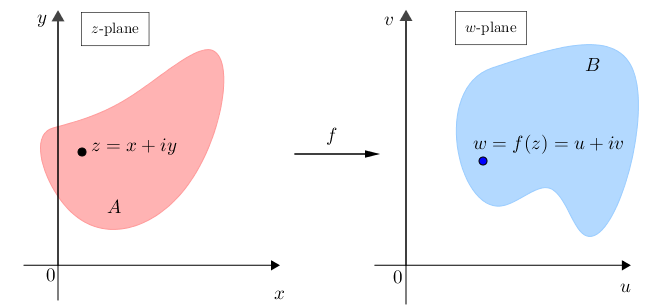
\includegraphics[scale=0.7]{transformacion.png}
\end{center}

\section{Tipos de Transformaciones}
Transformaciones hay infinitas, cada funci\'on compleja existente es una transformaci\'on. Y las hay de todo tipo. Pero las m\'as elementales son f\'aciles de reconocer, y con reconocer me refiero a saber c\'omo mapean ciertas regiones o curvas del plano $\mathbb{C}_z$ a $\mathbb{C}_w$. Analizaremos sobre todo las transformaciones debido a las funciones elementales ya vistas anteriormente, y algunas m\'as.

\subsection{Escalado y Rotaci\'on}
Una transformaci\'on que es capaz de escalar (es decir, tanto dilatar como contraer) y rotar regiones en el plano complejo respecto al origen est\'a dado por $$w = Az, \qquad A \in \mathbb{C}$$

Si consideramos que $A=ae^{i\alpha}$ y $z = re^{i\theta}$, entonces demostramos los efectos de dicha transformaci\'on:
\begin{eqnarray*}
w &=& Az\\
w &=& ae^{i\alpha}\ re^{i\theta} \\
w &=& ar\ e^{i(\alpha + \theta)}
\end{eqnarray*}
Con este desarrollo vemos que: $$|w| = ar \qquad \qquad \arg w = \alpha + \theta$$

Esto quiere decir que al complejo original $z$ el m\'odulo se escal\'o por un factor $a = |A|$ y se lo rot\'o gr\'aficamente una cantidad $\alpha = \arg A$. Tenemos adem\'as que:
\begin{itemize}
	\item Si $|A|>1$ se produce una dilataci\'on, mientras que si $|A|<1$ se produce una contracci\'on.
	\item Si $|A|=1$, es decir, $A$ pertenece a la circunferencia unitaria, no se produce escalado alguno, el m\'odulo de $z$ permanece intacto.
	\item Si $\arg A > 0$ se rota al complejo en sentido antihorario, y si $\arg A < 0$ ser\'a en sentido horario.
	\item Si $\arg A = 0$, es decir, $A$ es un real positivo, $z$ no se rota en absoluto.
\end{itemize}


\colorbox{green!40!white!80}{\parbox{\linewidth}{
 \theoremstyle{definition}
 \begin{definition}{Transformaci\'on de escalado y rotaci\'on}\\
  	Llamaremos \textbf{transformaci\'on de escalado y rotaci\'on} a la aplicaci\'on $f: \mathcal{S} \subset \mathbb{C} \rightarrow \mathbb{C}$ tal que: $$f(z) = Az$$ Donde $A \in \mathbb{C}$ es una constante compleja cualquiera, cuyo m\'odulo define en cu\'anto se escala la imagen, y cuyo argumento determina en cu\'anto se rota respecto al origen (siempre alrededor de $z=0$).
 \end{definition}}}
\linebreak
\linebreak

\begin{center}
	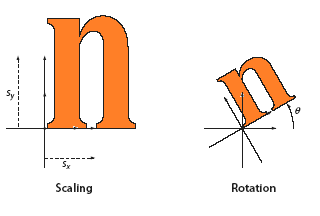
\includegraphics[scale=1]{scale_rot.png}
\end{center}


\subsection{Traslaci\'on}
Una transformaci\'on que traslada de manera intacta regiones en el plano viene dada de la forma m\'as simple de todas: $$w = z + B \qquad B \in \mathbb{C}$$

Si consideramos $B = a + ib$ y $z = x + iy$, entonces demostramos los efectos de dicha transformaci\'on:
\begin{eqnarray*}
w &=& z + B\\
w &=& (x + iy) + (a + ib)\\
w &=& (x + a) + i(y + b)
\end{eqnarray*}
Con este desarrollo vemos que $$\mathfrak{Re}(w) = x+a \qquad \qquad \mathfrak{Im}(w)=y+b$$

Esto quiere decir que al complejo original $z$ se lo desplaz\'o gr\'aficamente $a$ unidades en sentido positivo del eje real, y $b$ unidades en sentido positivo del eje imaginario. Tenemos adem\'as que:
\begin{itemize}
	\item Si $\mathfrak{Re}(B) > 0$ se produce un desplazamiento de $z$ hacia la derecha, y si  $\mathfrak{Re}(B) < 0$, ser\'a hacia la izquierda.
	\item Si $\mathfrak{Re}(B) = 0$ no hay desplazamiento horizontal.
	\item Si $\mathfrak{Im}(B) > 0$ se produce un desplazamiento de $z$ hacia arriba, y si  $\mathfrak{Im}(B) < 0$, ser\'a hacia abajo.
	\item Si $\mathfrak{Im}(B) = 0$ no hay desplazamiento vertical.
\end{itemize}


\colorbox{green!40!white!80}{\parbox{\linewidth}{
 \theoremstyle{definition}
 \begin{definition}{Transformaci\'on de traslaci\'on}\\
  	Llamaremos \textbf{transformaci\'on de traslaci\'on} a la aplicaci\'on $f: \mathcal{S} \subset \mathbb{C} \rightarrow \mathbb{C}$ tal que: $$f(z) = z+B$$ Donde $B \in \mathbb{C}$ es una constante compleja cualquiera, cuya parte real define en cu\'anto se desplaza horizontalmente el resultado, y cuya parte imaginaria determina el desplazamiento vertical.
 \end{definition}}}
\linebreak

\begin{center}
	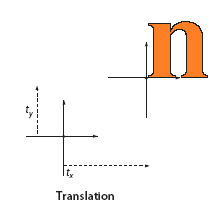
\includegraphics[scale=1]{translation.png}
\end{center}


\subsection{Transformaci\'on lineal}
Englobaremos a ambas transformaciones anteriores para definir lo que denominamos \textbf{Transformaci\'on lineal} o tambi\'en \textbf{Transformaci\'on af\'in}: $$w = Az + B \qquad A,B \in \mathbb{C}$$
\'Esta es una transformaci\'on capaz de escalar a $z$, rotarlo en torno al origen, y trasladarlo, acorde a la naturaleza de las constantes $A$ y $B$ como se detall\'o previamente.\\

\colorbox{green!40!white!80}{\parbox{\linewidth}{
 \theoremstyle{definition}
 \begin{definition}{Transformaci\'on lineal}\\
  	Llamaremos \textbf{transformaci\'on lineal} o \textbf{transformaci\'on af\'in} a la aplicaci\'on $f: \mathcal{S} \subset \mathbb{C} \rightarrow \mathbb{C}$ tal que $f(z)$ sea la composici\'on de las aplicaciones de traslaci\'on ($T = z + B$) con la de escalado-rotaci\'on ($E=Az$): $$f(z) = T \circ E\ (z) = Az + B$$
  	 Donde $A,B \in \mathbb{C}$ son constantes complejas, con  $A\neq 0$. El complejo $A$ determina la naturaleza de la rotaci\'on y escalado, y $B$ la de traslaci\'on.
 \end{definition}}}
\linebreak
\linebreak

\subsection{Inversi\'on}
Ahora analizaremos a una de las m\'as fascinantes transformaciones elementales, la \textbf{transformaci\'on rec\'iproca} o \textbf{inversa}: $$w = \frac{1}{z} \qquad z \neq 0$$
Se preguntar\'an ?`qu\'e es lo que hace? Bueno, la respuesta viene dada por un peque\~no an\'alisis de la misma:
\begin{eqnarray*}
w &=& \frac{1}{z}\\
w &=& \frac{1}{re^{i\theta}}\\
w &=& \frac{1}{r}e^{-i\theta}\\
\end{eqnarray*}
Con este desarrollo vemos que: $$|w| = \frac{1}{r} \qquad \qquad \arg w = -\theta$$

Esto quiere decir que se invirti\'o el m\'odulo del complejo $z$ y luego se lo reflej\'o respecto del origen. Tenemos las siguientes caracter\'isticas:

\begin{multicols}{2}
\begin{itemize}
	\item Consid\'erese la circunferencia unitaria $|z| = 1$. Si $|z|>1$, es decir $z$ est\'a fuera de la circunferencia unitaria, la funci\'on la mapea dentro de ella. En caso de que $|z|<1$, es decir $z$ dentro de la circunferencia unitaria, la funci\'on la mapea afuera.
	\item Si $|z|=1$, es decir $z$ sobre la circunferencia unitaria, no hay efecto de escalado alguno.
	\item Como $\arg w = - \arg z$, el complejo se reflejar\'a respecto al eje real.
\end{itemize}

\begin{center}
	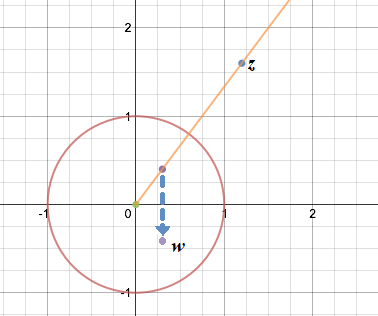
\includegraphics[scale=0.8]{inverse.png}
\end{center}

\end{multicols}

\colorbox{green!40!white!80}{\parbox{\linewidth}{
 \theoremstyle{definition}
 \begin{definition}{Transformaci\'on inversa}\\
  	Llamaremos \textbf{transformaci\'on inversa} o \textbf{rec\'iproco} a la aplicaci\'on $f: \mathcal{S} \subset \mathbb{C} \rightarrow \mathbb{C}$ tal que $$f(z) = \frac{1}{z} \qquad z\neq0$$

 \end{definition}}}
\linebreak
\linebreak

Bajo esta transformaci\'on, las rectas se convierten en c\'irculos, y los c\'irculos en rectas. Ni las rectas m\'as derechas ni las curvas m\'as cerradas se pueden resistir a la transformaci\'on inversa...\\
\begin{center}
	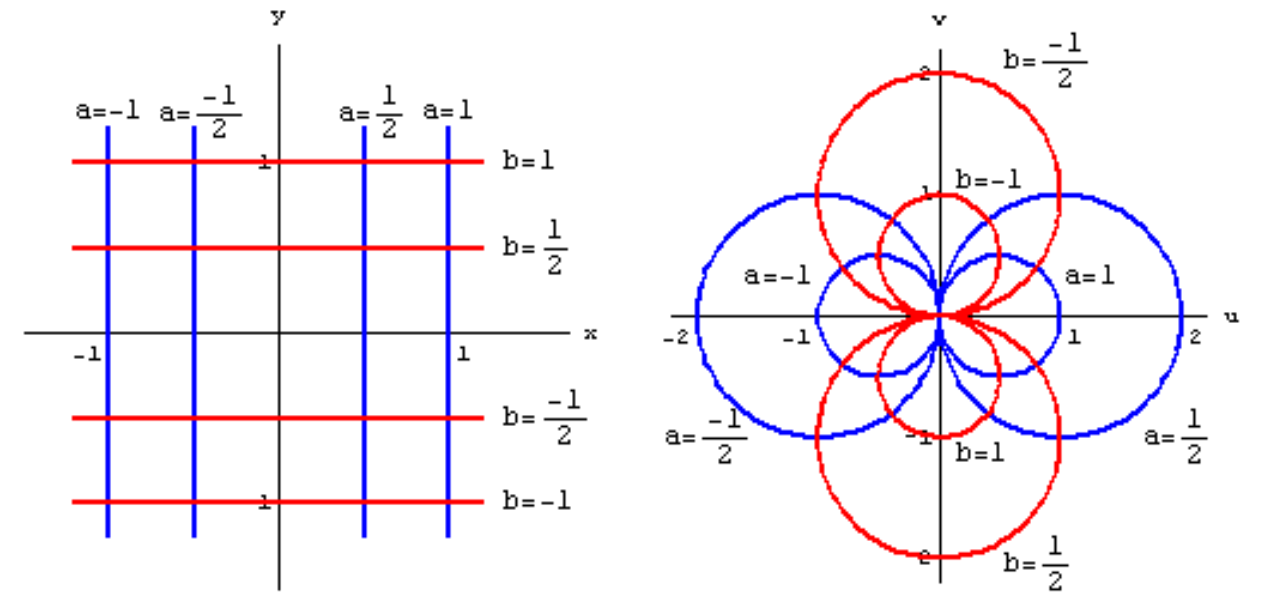
\includegraphics[scale=0.5]{reciprocal.png}
\end{center}

%Si consideramos la forma m\'as gen\'erica de la transformaci\'on inversa: $$w = \frac{1}{A(z-B)} = \frac{1}{Az - AB} \qquad A,B \in \mathbb{C}\: \land \: z\neq -B$$
%Podemos correr el centro de inversi\'on al punto $z_0 = B$ y establecer el l\'imite de inversi\'on en la circunferencia centrada en $z_0$ con radio $r = \frac{1}{\sqrt{|A|}}$, adem\'as de a\~nadir una rotaci\'on en sentido antihorario de magnitud $\theta = \arg (\frac{1}{\sqrt{A}})$

\subsection{Transformaci\'on de M\"obius}\
Combinando la transformaci\'on lineal y la transformaci\'on inversa, tenemos la denominada \textbf{transformaci\'on racional lineal} o \textbf{Transformaci\'on de M\"obius}: $$w = \frac{Az + B}{Cz + D} \qquad A, B,C,D \in \mathbb{C}\: \land\: AD - CB \neq 0$$

Tal transformaci\'on puede, seg\'un los valores que se les asigne a las constantes, inducir una rotaci\'on, un escalado, traslaci\'on e inclusive inversi\'on de $z$. Es \'esta la m\'as abarcativa de las transformaciones. Puede curvar a las m\'as r\'igidas de las rectas y enderezar a las m\'as duras de las circunferencias.\\

Si $C=0$, la transformaci\'on anterior se reduce a una simple transformaci\'on lineal. Pero si $C\neq 0$, la transformaci\'on de M\"obius puede definirse en t\'erminos de la composici\'on de todas las transformaciones antes vistas: $$w = \frac{A}{C} + \frac{BC - AD}{C} \cdot \frac{1}{Cz+D}$$
Donde se sigue exigiendo, claro est\'a, que $AD-CB \neq 0$.\\

Por el hecho de que la Transformada de M\"obius se puede expresar de la forma $$azw + bz + cw+d =0$$ se la llama tambi\'en \textbf{transformaci\'on bilineal}, al demostrarse que es lineal con respecto a $z$ y con respecto a $w$ (los coeficientes son complejos distintos a los presentados en la funci\'on anterior). Dicho esto, se puede tranquilamente despejar $z$ y obtener la transformada inversa, la cual es una transformaci\'on de la misma naturaleza: $$z = \frac{-Dw+B}{Cw-A} \qquad AD-BC\neq0$$

\colorbox{green!40!white!80}{\parbox{\linewidth}{
 \theoremstyle{definition}
 \begin{definition}{Transformaci\'on de M\"obius}\\
  	Llamaremos \textbf{transformaci\'on de M\"obius} o \textbf{racional lineal} o \textbf{bilineal} a la aplicaci\'on $f: \mathcal{S} \subset \mathbb{C} \rightarrow \mathbb{C}$ tal que $$f(z) = \frac{Az+B}{Cz+D} \qquad z\neq -\frac{D}{C}$$
En donde $A,B,C,D \in \mathbb{C}$ y debe darse que $AD-BC\neq 0$
 \end{definition}}}
\linebreak
\linebreak

Bajo una transformaci\'on de M\"obius, las curvas en el plano (a) se transforman en las curvas correspondientes en el plano (b) en la siguiente figura:\\
\begin{center}
	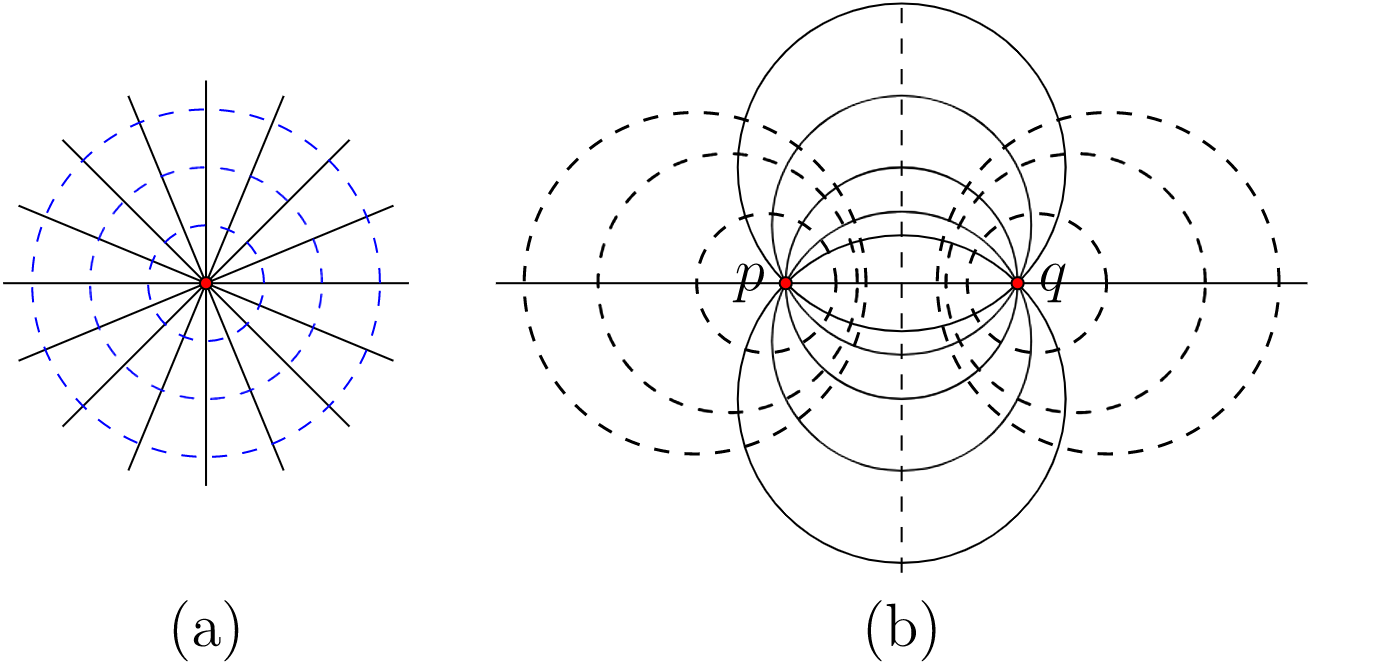
\includegraphics[scale=0.4]{moebius_transformation.png}
\end{center}

%\subsection{Transformaci\'on exponencial y logar\'itmica}
%//pass

%\subsection{Transformaciones trigonom\'etricas}
%//pass

%\subsection{Transformaci\'on $w = z^n$}
%//pass


\section{Parametrizando curvas en $\mathbb{C}$}
En c\'alculo de varias variables se parametrizan curvas haciendo que una funci\'on $f: \mathbb{R}^2 \rightarrow \mathbb{R}$ tome como variables $x(t), y(t)$, ambos dependientes a su vez de un par\'ametro adicional en com\'un. Se lo llamaba $t$ por asociarlo com\'unmente con el tiempo, en aplicaciones f\'isicas.

Se ha hecho notar ya la asombrosa similitud entre funciones de dos variables reales y funciones complejas. El hecho de que un n\'umero complejo $z$ represente un punto en el plano $\mathbb{C}$ es lo que nos demuestra que hay una correlaci\'on un\'ivoca con $\mathbb{R}^2$. Las componentes real e imaginaria de un complejo se correlacionan inconfundiblemente con las coordenadas del mism\'isimo $\mathbb{R}^2$. Entonces, si hablamos de parametrizar curvas en el plano de Argand, o plano complejo, tendr\'iamos que definir un n\'umero complejo $z$ cuyos componentes real e imaginario sean funciones respecto a una variable real cualquiera $t$.

$$\mathcal{C}:\: z = z(t) \qquad a \leq t \leq b$$
$$z(t) = x(t) + i\ y(t)$$

\colorbox{orange!40!white!80}{\parbox{\linewidth}{
 \theoremstyle{definition}
 \begin{definition}{Arco suave}\\
  	Dada la curva $\mathcal{C}:\: z = z(t)$ en donde $a \leq t \leq b$ y $z(t) = x(t) + i\ y(t)$, se dice que $\mathcal{C}$ es un \textbf{arco suave} si:
  	\begin{itemize}
  		\item $x(t), y(t)$ son funciones inyectivas en el intervalo $I=[a,b]$
  		\item $x'(t), y'(t)$ son funciones continuas en $I$
  		\item $z'(t)\neq 0$ en $I$
  	\end{itemize}
 \end{definition}}}
\linebreak
\linebreak

B\'asicamente hablando, una curva no ser\'a suave si:
\begin{enumerate}
	\item Se corta a s\'i misma
	\item Presenta crestas o picos
	\item Permanece en un mismo punto al ser evaluada en un intervalo de su dominio.\\
\end{enumerate}


\colorbox{orange!40!white!80}{\parbox{\linewidth}{
 \theoremstyle{definition}
 \begin{definition}{\'Angulo entre curvas en el Plano Complejo}\\
  	Sean $\mathcal{C}_1, \mathcal{C}_2$ dos arcos suaves simples en una regi\'on $\mathcal{D} $ del plano complejo que se interceptan en un punto $z_0$. Se denomina \'angulo entre $\mathcal{C}_1$ y $\mathcal{C}_2$ en $z_0$ al \'angulo formado por las respectivas rectas tangentes en dicho punto.
  	
 \end{definition}}}
\linebreak
\linebreak


\section{La Transformaci\'on Conforme}
De todas las transformaciones existentes, les cuento el secreto... las estrellas del espect\'aculo son aquellas que al transformar varias curvas, logran conservar el m\'as simple de los detalles: el \'angulo entre ellos.\\


\colorbox{red!40!white!80}{\parbox{\linewidth}{
 \theoremstyle{definition}
 \begin{definition}{Transformaci\'on que preserva la orientaci\'on}\\
  	Sea $f: \mathcal{D} \subset \mathbb{C} \rightarrow \mathcal{S}\subset \mathbb{C}$. Diremos que $f$ conserva la orientaci\'on si una rotaci\'on en sentido antihorario en $\mathcal{D}$ se transforma por $f$ en una rotaci\'on en sentido antihorario en $\mathcal{S}$.

 \end{definition}}}
\linebreak
\linebreak

\colorbox{red!40!white!80}{\parbox{\linewidth}{
 \theoremstyle{definition}
 \begin{definition}{Transformaci\'on que preserva los \'angulos}\\
  	Sea $f: \mathcal{D} \subset \mathbb{C} \rightarrow \mathcal{S}\subset \mathbb{C}$. Diremos que $f$ conserva los \'angulos si para cualquier $z_0 \in \mathcal{D}$, dados dos arcos cualesquiera que se intersectan en $z_0$ formando un \'angulo $\alpha$, las im\'agenes de estas curvas se cortan en $f(z_0) \in \mathcal{S}$ formando entre s\'i el mismo \'angulo $\alpha$.

 \end{definition}}}
\linebreak
\linebreak

Dadas estas dos definiciones, ahora les presentamos, se\~noras y se\~nores, a la estrella del cap\'itulo: las \textbf{Transformaciones Conforme}\\

\colorbox{red!40!white!80}{\parbox{\linewidth}{
 \theoremstyle{definition}
 \begin{definition}{Transformaci\'on Conforme}\\
  	Sea $f: \mathcal{D} \subset \mathbb{C} \rightarrow \mathcal{S}\subset \mathbb{C}$. La transformaci\'on $w = f(z)$ se dice que es \textbf{una transformaci\'on conforme} en un punto $z_0 \in \mathcal{D}$ si preserva el \'angulo entre curvas que se interceptan en $z_0$ tanto en magnitud como orientaci\'on.

 \end{definition}}}
\linebreak

\begin{multicols}{2}
La importancia de las llamadas transformaciones conforme radica en su utilidad para resolver problemas en el campo de la f\'isica, qu\'imica, ingenier\'ia y matem\'aticas en general, entre tantos otros, que pueden ser expresados en t\'erminos de variable compleja pero que presentan severas dificultades en su geometr\'ia. Las trasformaciones se utilizan con el objetivo de simplificar tales problemas.

\begin{center}
	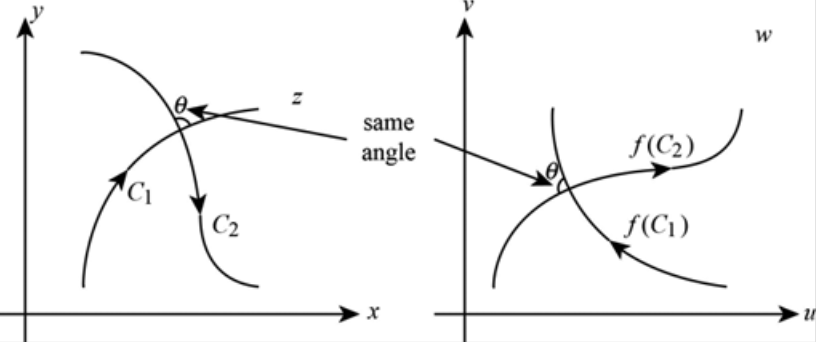
\includegraphics[scale=0.39]{conformal.png}
\end{center}
\end{multicols}

Asociado a un gran concepto siempre viene un gran teorema...\\

\colorbox{magenta!40!white!80}{\parbox{\linewidth}{
\theoremstyle{theorem}
\begin{theorem} {Condici\'on Suficiente para la Conformidad}\\
Sea $f: \mathcal{D} \subset \mathbb{C} \rightarrow \mathcal{S}\subset \mathbb{C}$.\\
Si $f$ es anal\'itica en $\mathcal{D}$ y $f'(z)\neq 0 \;\forall z \in \mathcal{D}$, entonces $f$ es conforme en $\mathcal{D}$.
\end{theorem}}}

Demostrar

\begin{center}
	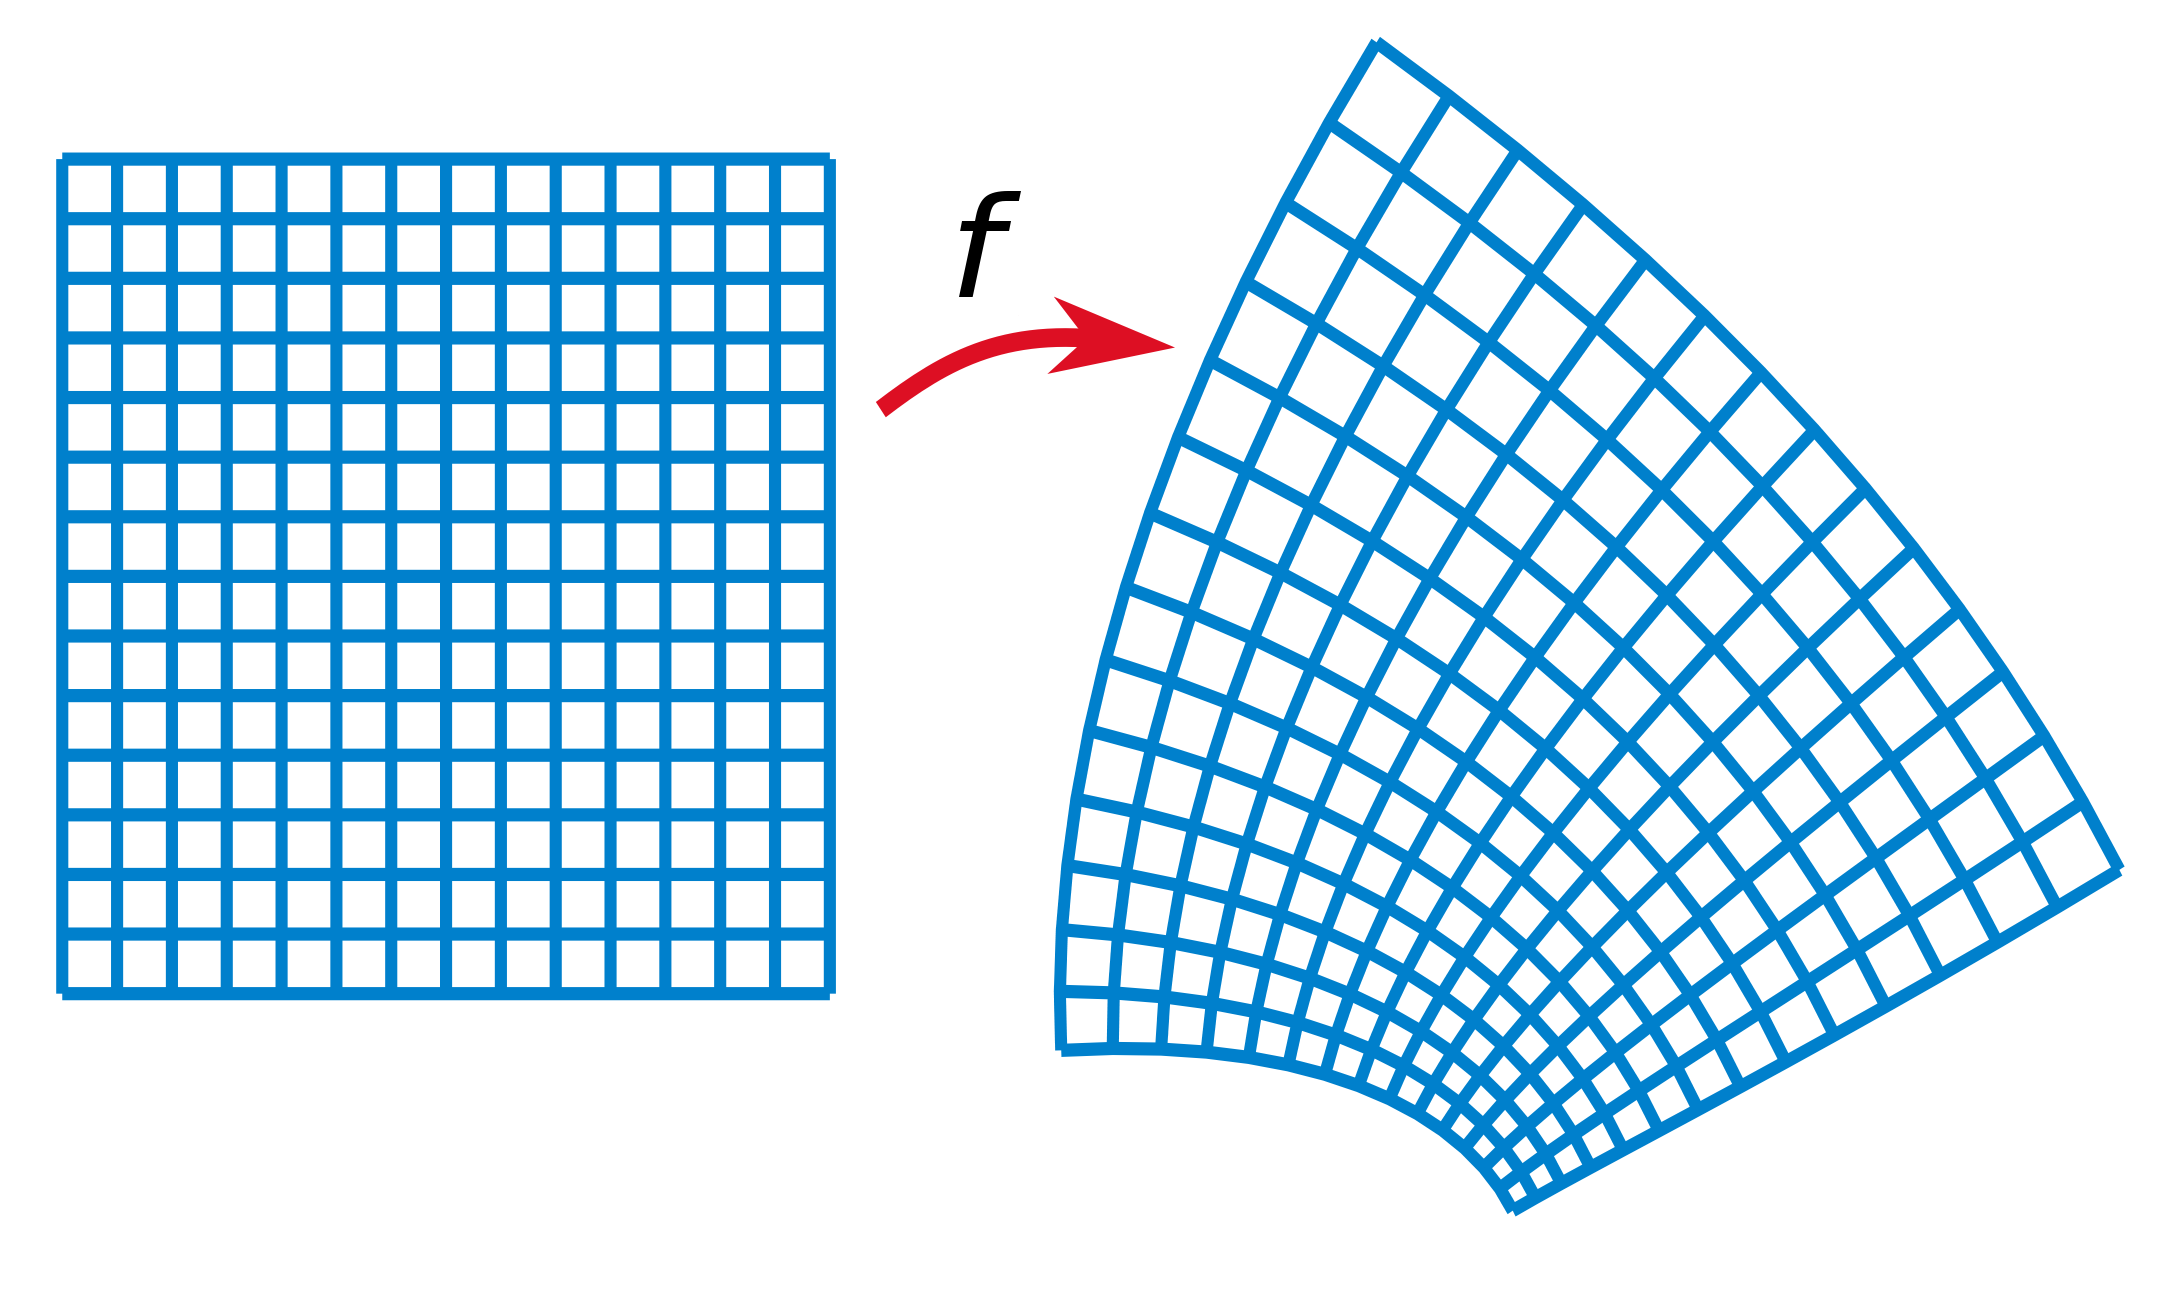
\includegraphics[scale=0.27]{conforme.png}\\
	\textit{Punto por punto, curva por curva, regi\'on por regi\'on, transformaremos \'areas enteras del plano complejo, revelando patrones incre\'ibles que ni en sue\~nos se nos presentar\'ian.}\\
\end{center}

\subsection{Aplicaci\'on}
Para los que crean que las transfomaciones conformes son aburridas, divi\'ertanse encontr\'andole sentido al procesamiento de im\'agenes con el mapeo conformacional...

\begin{center}
	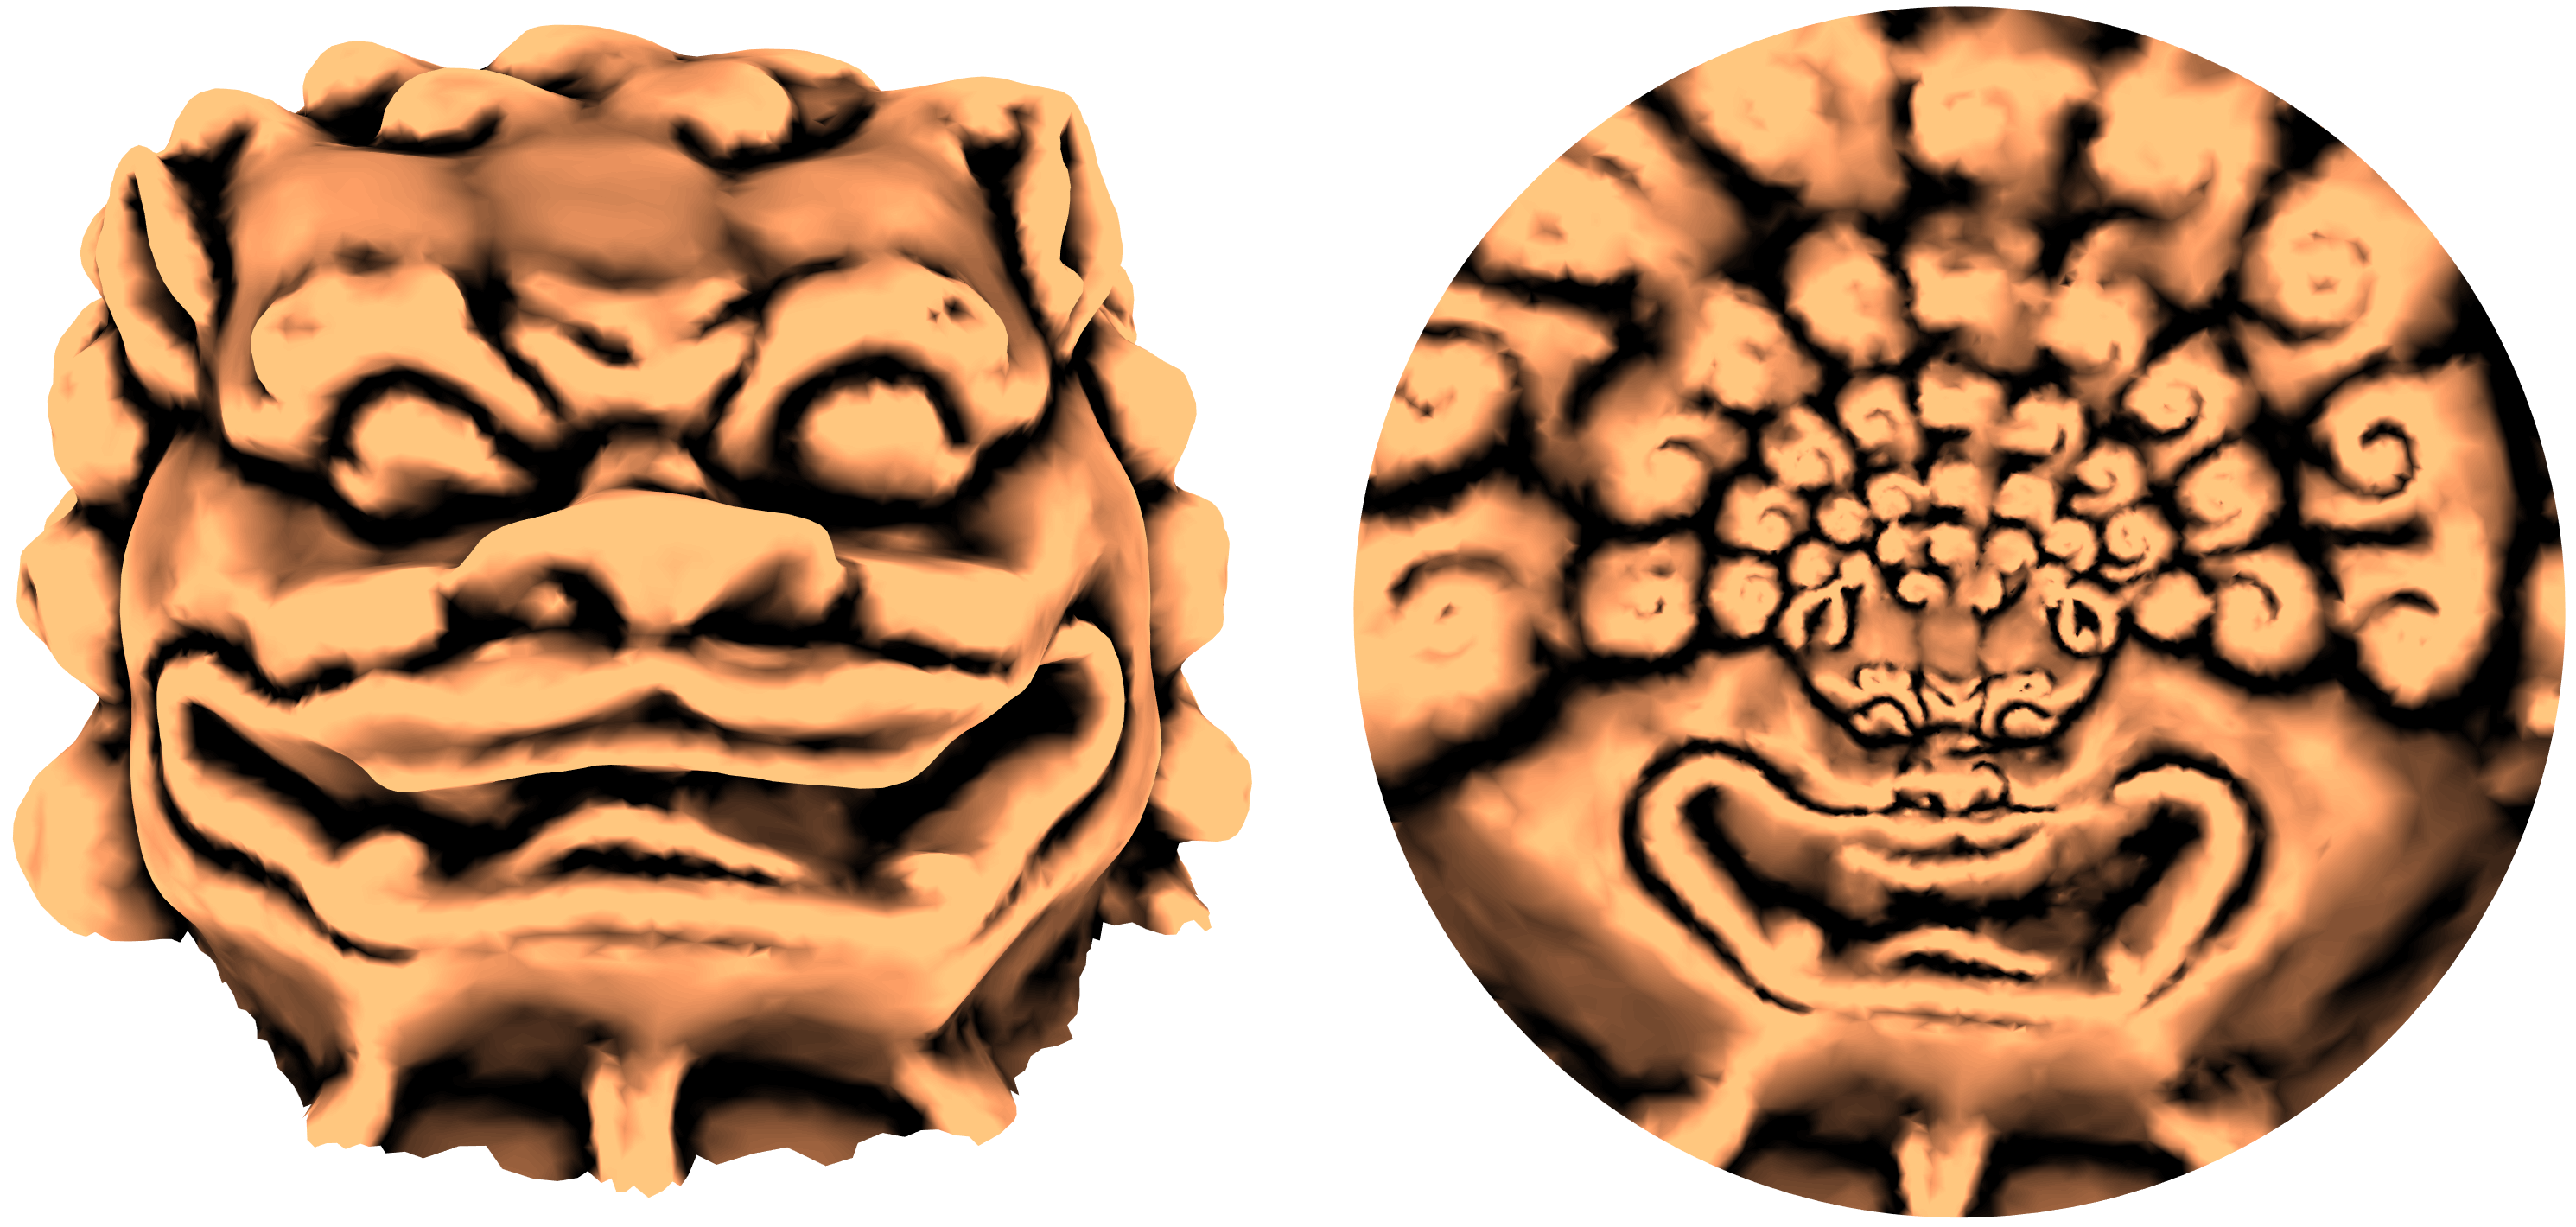
\includegraphics[scale=0.4]{matlab_conformal.png}
\end{center}

\end{document}